% Shared preamble for the English summaries in this repository.
\documentclass[11pt,a4paper]{article}
\usepackage[margin=2.2cm]{geometry}
\usepackage[T1]{fontenc}
\usepackage[utf8]{inputenc}
\usepackage{lmodern}
\usepackage{amsmath,amssymb}
\usepackage{graphicx}
\usepackage{booktabs}
\usepackage{enumitem}
\usepackage[hidelinks]{hyperref}
\setlist{itemsep=2pt,topsep=4pt}
\setlength{\parindent}{0pt}
\setlength{\parskip}{5pt}
\graphicspath{{figures/}}
\newcommand{\summaryheader}[3]{%
  \begin{center}
    {\Large\bfseries #2}\\[3pt]
    {\large #1}\\[3pt]
    {\small Arshia Goshtasbi \textbullet{} MSc Electrical Engineering (Control), Iran University of Science and Technology \textbullet{} #3}
  \end{center}
  \vspace{2pt}\hrule\vspace{8pt}\par}

\begin{document}
\summaryheader{Machine Learning, Homework 4}{Feature Selection and Dimensionality Reduction}{Spring 1404 (2025)}

\textbf{Notebook} (\texttt{breast\_cancer\_features.ipynb}). The data are the Wisconsin diagnostic breast-cancer data: 569 samples, 30 features, malignant or benign.
\begin{itemize}
  \item \emph{SelectKBest} ($F$-test) kept the size and concavity features (radius, perimeter, area, concavity, concave points; mean and worst values).
  \item \emph{RFE} with logistic regression kept a different set, including texture, smoothness, compactness and symmetry terms. RFE ranks features by their weight in a multivariate model, while the $F$-test scores each feature alone, so correlated size features are not all kept by RFE.
  \item A \emph{random forest} gave feature importances; Figure~\ref{fig:hw4} shows the top ten.
  \item \emph{PCA} to two components explains $99.8\%$ of the variance. This is because the features were not standardised, so the area features (values in the hundreds to thousands) dominate. \emph{t-SNE} separates the classes more clearly than this PCA projection.
\end{itemize}

\begin{figure}[h]\centering
  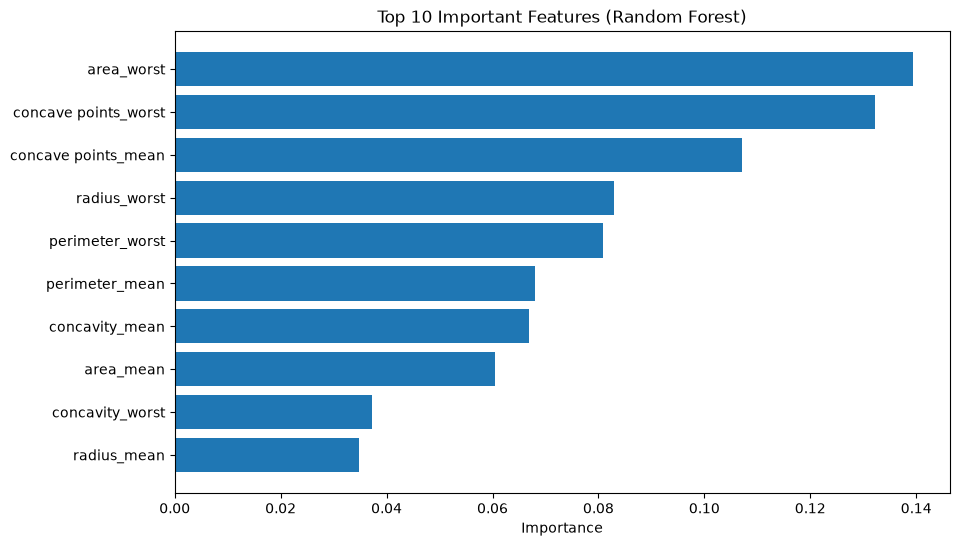
\includegraphics[width=.48\linewidth]{breast_cancer_features_cell10_1.png}\hfill
  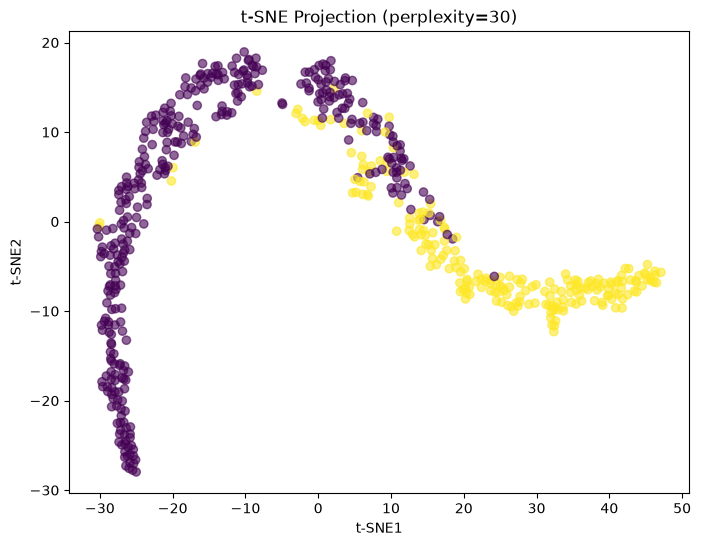
\includegraphics[width=.48\linewidth]{breast_cancer_features_cell15_1.png}
  \caption{Random-forest importances (left) and t-SNE embedding coloured by diagnosis (right).}\label{fig:hw4}
\end{figure}

\textbf{Written part.}
\begin{description}
  \item[PCA of three points.] For $(1,1),(0,0),(-1,-1)$ the mean is $0$ and the first principal axis is $(1,1)/\sqrt2$. The projections are $\sqrt2,0,-\sqrt2$, with variance $4/3$ (dividing by $n$). The points lie on that axis, so the reconstruction error is zero.
  \item[PCA vs.\ Fisher LDA.] PCA keeps the direction of largest spread and ignores labels. LDA picks the direction that best separates the two classes, so it can differ from PCA.
  \item[Forward and backward search.] I explained greedy forward selection and wrote the backward version: start from all $K$ features and, at each step, remove the feature whose removal increases the validation error least.
  \item[Knapsack.] Choosing features under a budget is like a knapsack problem and resembles wrapper methods. Dynamic programming finds the global optimum for small integer instances, but the problem is NP-hard, so large instances use greedy heuristics without that guarantee.
  \item[PCA and kernel PCA] of four points in $\mathbb R^4$ projected to one dimension; for kernel PCA with $k(x,y)=(x^\top y)^2$ I eigen-decomposed the $4\times4$ Gram matrix.
\end{description}
\end{document}
